%%Bài toán đề xuất bởi NVPL

\textbf{Tương tác tĩnh điện của protein}

Nghiên cứu về vật lý trong sinh học đã trở thành một trong những chủ đề bùng nổ và hấp dẫn gần đây, trong số đó có chủ đề mà bài toán này tìm hiểu, đó là tương tác tĩnh điện của protein trong DNA với điện tích trong môi trường nước hoặc trong môi trường có ion tự do (môi trường chứa muối đơn trị như NaCl) để giải thích một số quá trình như \textit{đảo điện tích (charge inversion)} trong hệ thống polyelectrolyte-micelle hay trên bề mặt rắn của màng mica hoặc lipid; hay hiện tượng \textit{điện di (electrophoresis)} trong quá trình sinh học (Ví dụ như quá trình chuyển gen đến tế bào sống với mục đích trị liệu gen,...).

\begin{enumerate}
    \item \textbf{Axit amin trong protein.} \\
    Đầu tiên ta tìm hiểu tại sao sâu bên trong protein, axit amin ion hoá lại hầu như không tích điện. Ta xét mô hình đơn giản của một điện tích, giả thiết như một quả cầu bán kính $R\approx 1.5\ \si{\angstrom}$, tích điện $q=\text{e}\approx 1.6 \times 10^{-19}\ \si{C} $, di chuyển từ môi trường nước bên ngoài protein vào sâu bên trong protein. Protein và nước coi như môi trường điện môi đồng nhất với hằng số điện môi lần lượt là $\epsilon_p \approx 3$, $\epsilon_w \approx 80$. Cho biết năng lượng tĩnh điện cần để phá huỷ bất kỳ cấu trúc protein nào xấp xỉ $E_0 \approx 5\ \si{kcal/mol}$ $(1\ \si{J} \approx 1.44 \times 10^{20}\ \si{kcal/mol})$.\\ \textit{Lưu ý: Trong toàn bộ bài tập này ta sẽ chủ yếu dùng đơn vị $\si{kcal/mol}$ cho năng lượng vì trong nghiên cứu về tế bào chủ yếu sử dụng đơn vị này nhưng vẫn chấp nhận kết quả bằng đơn vị Joule.}\\ \\
    Xác định độ chênh lệch năng lượng tĩnh điện của một điện tích nếu điện tích đó xuất hiện bên trong protein. Vậy tại sao axit amin ion hoá lại hầu như không tích điện bên trong protein ?

    \item \textbf{Tương tác giữa điện tích và protein trong môi trường nước.} \\
    \begin{center}
    \begin{figure}[htp]
    \begin{center}
        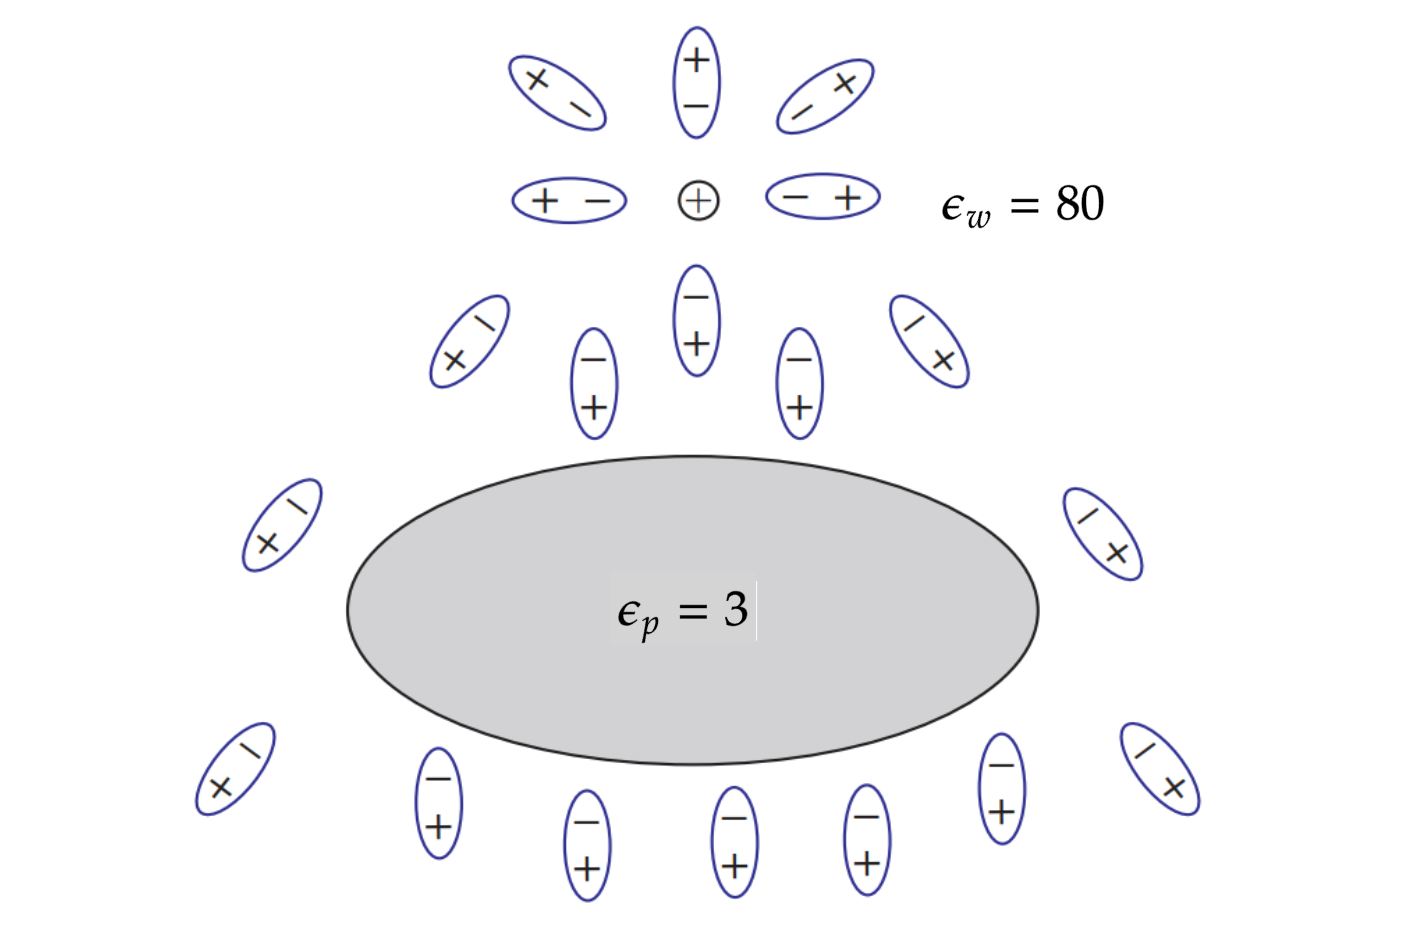
\includegraphics[scale=.23
        ]{Problem_13/image/1.png}
    \end{center}
    \begin{center}
    Hình 1: Các lưỡng cực bị phân cực
    \end{center}
    \end{figure}
\end{center}
    Tiếp đến ta tính tương tác của các điện tích ở gần hay tại mặt phân cách của protein và nước \textbf{(Hình 1)}. Coi điện tích rất bé và nằm rất gần so với protein để có thể mô hình hoá protein như một tấm điện môi đồng nhất có hai mặt phẳng rộng vô hạn song song với nhau \textbf{(Hình 2)}. Trong từng vùng môi trường, tồn tại "hằng số điện môi hiệu dụng" $\epsilon_{\text{eff}}$, cho phép tính điện thế của điện tích $q$ gây ra tại vị trí $\Vec{r}$ rất xa so với chính nó (nhưng đủ lớn để không coi điện thế bằng $0$) như thể điện tích $q$ được đặt trong môi trường điện môi đồng nhất có hằng số điện môi bằng hằng số điện môi hiệu dụng:$$V(\Vec{r})=\dfrac{kq^2}{\epsilon_{\text{eff}}\left|\Vec{r}\right|}.$$ Do vùng không gian môi trường nước chứa điện tích, các lưỡng cực phân cực mạnh hơn vùng không gian không chứa điện tích nên khi ta khảo sát tương tác tĩnh điện đối với mặt phân cách gần điện tích thì ảnh hưởng của mặt phân cách xa điện tích là không đáng kể. Ngoài ra khi khảo sát tĩnh điện ở vùng không gian môi trường nước không chứa điện tích, các lưỡng cực trong nước bị phân cực mạnh hơn trong protein nên ta chỉ xét ảnh hưởng của các điện tích liên kết trong môi trường nước ở mặt phân cách xa điện tích. Do đó ta gần đúng hệ này bằng cách tách thành hai hệ tương tác tĩnh điện giữa điện tích điểm $q$ hoặc $q''$ và mặt phẳng điện môi bán vô hạn \textbf{(Hình 2)}.
    \begin{center}
    \begin{figure}[htp]
    \begin{center}
        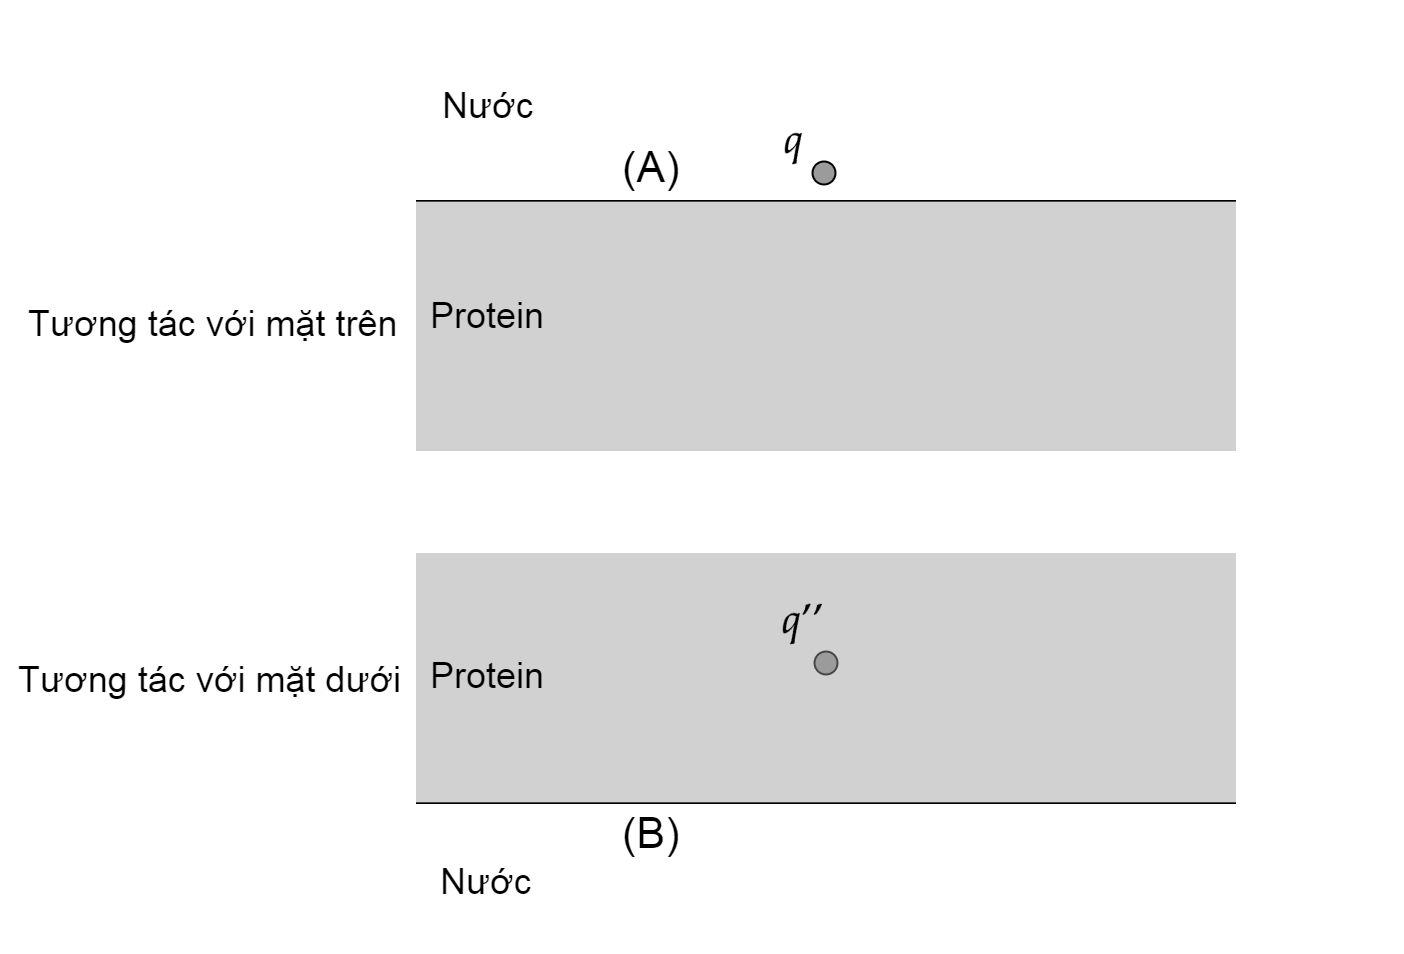
\includegraphics[scale=.27
        ]{Problem_13/image/2.png}
    \end{center}
    \begin{center}
    Hình 2: Tương tác giữa điện tích và protein trong từng môi trường. Điện tích $q$ là điện tích ban đầu ta xét. Điện tích $q''$ là điện tích ảnh sinh ra do sự tương tự về mặt tĩnh điện của các điện tích liên kết trong môi trường protein.
    \end{center}
    \end{figure}
\end{center}

     \begin{enumerate}[label=\textbf{\alph*,}]\itemsep0em
        \item Xác định hằng số điện môi hiệu dụng trong vùng môi trường nước chứa điện tích.
        \item Xác định hằng số điện môi hiệu dụng trong vùng môi trường bên trong protein.
        \item Xác định hằng số điện môi hiệu dụng trong vùng môi trường nước không chứa chứa điện tích.
    \end{enumerate}

    \item \textbf{Tương tác giữa điện tích và protein trong môi trường có ion tự do.} \\ 
    Cho đến giờ ta mới chỉ tìm hiểu về tương tác giữa các điện tích riêng biệt. Tuy nhiên ta đã "bỏ sót" tương tác của các lưỡng cực (các lưỡng cực cũng tham gia vào liên kết hydro như $\text{H}^+ - \text{O}^-$ và $\text{H}^+ - \text{N}^-$) và cũng như các tứ cực (các vòng thơm) bên trong các cấu trúc tế bào. Thêm vào đó, do các điện tích tự do có sẵn trong nước (nước muối), từ những điều kể trên chúng ta rút ra biểu thức điện thế gây ra bởi điện tích $q$ tại vị trí $\Vec{r}$ rất xa so với chính nó (nhưng đủ lớn để không coi điện thế bằng $0$) có dạng: $$V(r)=\dfrac{kq}{\epsilon_{\text{eff}}}\dfrac{e^{-r/D}}{r}.$$Thế năng này gọi là thế "chắn" hay thế Debye-Huckel hay thế Yukawa, xuất hiện rất nhiều trong các lĩnh vực khác nhau của vật lý. Ở đây $D$ là bán kính "chắn" Debye-Huckel, tương ứng với kích thước điển hình của đám mây phản ion xung quanh điện tích. Giá trị của $D$ không phụ thuộc vào điện tích $q$ mà phụ thuộc hằng số điện môi hiệu dụng, nhiệt độ và cường độ ion (ionic strength) $I\ \si{mol/l}$ của dung dịch: $$I=\dfrac{1}{2}\sum\limits_i {{c_i}N_i^2}. $$ Trong đó $N_i$ là tỉ số giữa điện tích của ion loại $i\ (i=1,2,3,...)$ và điện tích nguyên tố. $c_i$ là nồng độ của ion loại $i$, tính bằng $\si{mol/l}$. Cho biết mật độ điện tích ion trong môi trường tuân theo phân bố Maxwell- Boltzmann: $$\rho(r)=\sum\limits_i {{c_i}\left( {\text{e}{N_i}} \right)} {e^{ - E_i/(k_BT)}}.$$ Giả thiết $E_i \ll k_BT$ ($T$ là nhiệt độ, $k_B$ là hằng số Boltzmann) và các ion coi như đứng yên. Hệ ion coi là trung hoà. Cho biết toàn bộ hệ ở nhiệt độ phòng $T=20 \si{^\circ C}$, hằng số điện môi hiệu dụng $\epsilon_{\text{eff}}=40$, cường độ ion $I \approx 0.12\ \si{mol/l}$. \\ \\
    Hãy xác định bán kính chắn Debye-Huckel của hệ.\\ \\
\textit{Có thể bạn cần dùng: $\nabla_r f(r)=\dfrac{1}{r}\dfrac{\partial}{\partial r}\Big(rf(r)\Big).$}


    
\end{enumerate}
\begin{flushright}
    (Biên soạn bởi Nhân viên phòng lab)
\end{flushright}